% Fig. 1 — C2D2 training overview (TikZ). Split from the architecture figure on the user's request (2026-11-13):
% Fig. 1 = how the model is trained (this file), Fig. 2 = the network (fig_arch.tex).
% Facts follow Section III-G (4_method.tex) and configs (TRAIN.QAF): each sensor corrupted with p = 0.5, one fifth of the
% corrupted sensors removed (zero-filled), one sensor-specific operator otherwise; curriculum x + c(x~ - x), c = 0.3/0.6/1.0
% from epochs 0/10/20 (DELIVER, MUSES); teacher = same architecture without the high-resolution path, trained on clean
% inputs, frozen, sees the clean input; KL weight beta = 0.5, T = 2; total loss L_clean + L_deg; inference = student once.
% Colours: carbon@11.84.0 (design-source: carbon@11.84.0), same tokens as fig_arch.tex.
\definecolor{cRGB}{HTML}{6929C4}
\definecolor{cDep}{HTML}{00539A}
\definecolor{cEvt}{HTML}{8E6A00}
\definecolor{cLid}{HTML}{9F1853}
\definecolor{acc}{HTML}{007D79}
\definecolor{ink}{HTML}{3C3838}
\definecolor{mut}{HTML}{565151}
\definecolor{bd}{HTML}{CAC5C4}
\definecolor{sf}{HTML}{F7F3F2}
\definecolor{g20}{HTML}{E5E0DF}
\begin{tikzpicture}[
  x=1cm, y=1cm, font=\sffamily\fontsize{6.5}{7.5}\selectfont, line cap=round, line join=round,
  >={Stealth[length=1.6mm, width=1.2mm]},
  flow/.style={->, draw=mut, line width=0.45pt},
  tflow/.style={->, draw=acc, line width=0.6pt},
  frozen/.style={draw=mut, dash pattern=on 1.6pt off 1.2pt, line width=0.45pt, fill=sf},
  trained/.style={draw=acc, line width=0.7pt, fill=white},
  plain/.style={draw=mut, line width=0.45pt, fill=white},
  ttl/.style={font=\sffamily\bfseries\fontsize{6.8}{8}\selectfont, text=ink},
  sub/.style={text=mut, font=\sffamily\fontsize{5.6}{6.6}\selectfont},
  plab/.style={font=\sffamily\bfseries\fontsize{8}{9}\selectfont, text=ink, anchor=west},
  dot/.style={circle, fill=mut, inner sep=0pt, minimum size=1.0mm},
]
% ---------- input stacks ----------
\newcommand{\stack}[3]{% #1 x, #2 y, #3 = 1 for degraded
  \foreach \f/\c/\k in {lidar/cLid/3, event/cEvt/2}{
    \node[inner sep=0pt] (s#3\k) at (#1+0.14*\k,#2+0.14*\k) {\includegraphics[width=0.95cm]{figures/fig1_thumbs/\f.png}};
    \draw[\c, line width=0.6pt] (s#3\k.south west) rectangle (s#3\k.north east);
  }
  \ifnum#3=0
    \node[inner sep=0pt] (s#31) at (#1+0.14,#2+0.14) {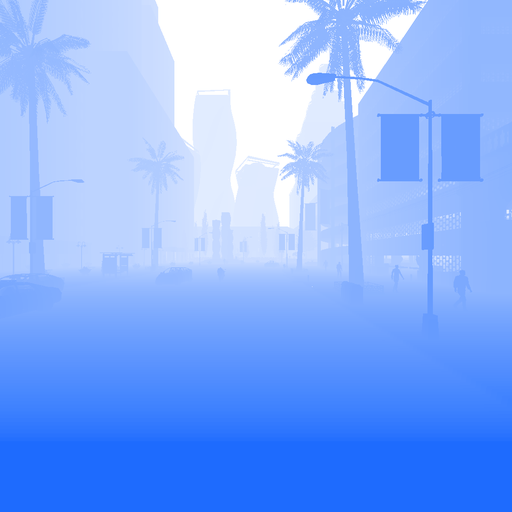
\includegraphics[width=0.95cm]{figures/fig1_thumbs/depth.png}};
    \draw[cDep, line width=0.6pt] (s#31.south west) rectangle (s#31.north east);
    \node[inner sep=0pt] (s#30) at (#1,#2) {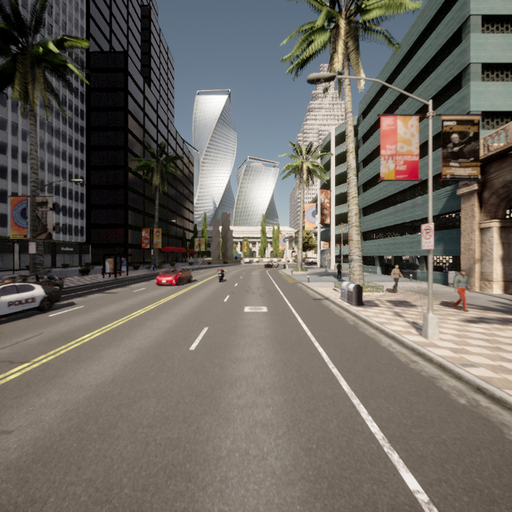
\includegraphics[width=0.95cm]{figures/fig1_thumbs/rgb.png}};
  \else
    \draw[cDep, line width=0.6pt, fill=white] (#1+0.14-0.475,#2+0.14-0.475) rectangle (#1+0.14+0.475,#2+0.14+0.475);
    \draw[cDep!60, line width=0.45pt] (#1+0.14-0.475,#2+0.14-0.475) -- (#1+0.14+0.475,#2+0.14+0.475);
    \node[inner sep=0pt] (s#30) at (#1,#2) {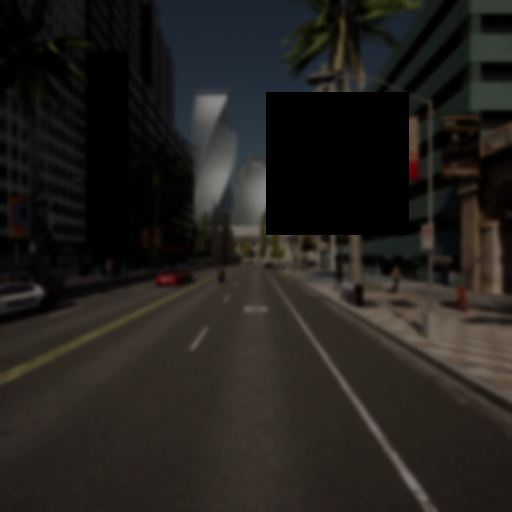
\includegraphics[width=0.95cm]{figures/fig1_thumbs/rgb_degraded.png}};
  \fi
  \draw[cRGB, line width=0.6pt] (s#30.south west) rectangle (s#30.north east);
}
\stack{1.0}{4.55}{0}
\node[sub, anchor=north] at (1.21,3.95) {clean training batch $x$};
\stack{1.0}{0.95}{1}
\node[sub, anchor=north, align=center] at (1.21,0.35) {degraded copy $\tilde{x}$};

% ---------- degradation ----------
\draw[flow] (0.75,3.3) -- (0.75,1.6);
\draw[plain, rounded corners=1.2pt] (2.3,1.35) rectangle (5.8,3.65);
\node[ttl, anchor=north west] at (2.42,3.57) {Sensor-specific degradation};
\node[sub, anchor=north west, align=left] at (2.42,3.24) {each sensor corrupted with $p=0.5$;\\one in five corrupted sensors removed\\(zero-filled), else one operator:};
\node[sub, anchor=north west, align=left] at (2.42,2.54) {%
\textcolor{cRGB}{RGB}: blur, gain, colour shift\\
\textcolor{cDep}{depth}: holes, scale change\\
\textcolor{cLid}{LiDAR}: dropped and jittered beams\\
\textcolor{cEvt}{event}: resolution loss; all: patch dropout};
\draw[mut, line width=0.45pt] (0.75,2.5) -- (2.3,2.5);
\node[dot] at (0.75,2.5) {};

% ---------- models ----------
% teacher (frozen) on top, fed by the clean batch
\draw[frozen, rounded corners=1.5pt] (6.2,5.65) rectangle (8.7,6.8);
\node[ttl] at (7.45,6.52) {Teacher $g$};
\node[sub, align=center] at (7.45,6.0) {frozen, clean-trained,\\no high-res.\ path};
\draw[mut, line width=0.45pt] (2.4,4.7) -- (2.4,6.25);
\node[dot] at (2.4,4.7) {};
\draw[flow] (2.4,6.25) -- (6.2,6.25);
\node[sub, anchor=south] at (4.3,6.27) {clean input only};
% student, clean pass
\draw[trained, rounded corners=1.5pt] (6.2,4.15) rectangle (8.7,5.25);
\node[ttl] at (7.45,4.9) {Model $\ell$ (Fig.~2)};
\node[sub] at (7.45,4.5) {clean pass};
\draw[flow] (1.9,4.7) -- (6.2,4.7);
% student, degraded pass
\draw[trained, rounded corners=1.5pt] (6.2,0.55) rectangle (8.7,1.65);
\node[ttl] at (7.45,1.3) {Model $\ell$ (Fig.~2)};
\node[sub] at (7.45,0.9) {degraded pass};
\draw[flow] (1.9,1.1) -- (6.2,1.1);
% shared weights
\draw[<->, draw=acc, line width=0.55pt, dash pattern=on 1.4pt off 1pt] (7.45,4.15) -- (7.45,1.65);
\node[sub, fill=white, inner sep=1.2pt, text=acc, align=center] at (7.45,2.9) {same weights,\\same batch};

% ---------- losses ----------
\node[anchor=west, text=ink, inner sep=1pt] (lc) at (9.2,4.7) {$\mathcal{L}_{\mathrm{clean}} = \mathcal{L}_{\mathrm{CE}}\big(\ell(x), y\big) + \text{aux.}$};
\draw[flow] (8.7,4.7) -- (lc.west);
\node[anchor=west, text=ink, inner sep=1pt] (ld) at (9.2,1.35) {$\mathcal{L}_{\mathrm{CE}}\big(\ell(\tilde{x}), y\big)$};
\node[anchor=west, text=acc, inner sep=1pt] (lk) at (9.2,0.7) {$+\,\beta\,\mathrm{KL}_T\big(g(x)\,\|\,\ell(\tilde{x})\big)$};
\draw[flow] (8.7,1.1) -- (8.95,1.1) |- (ld.west);
\draw[flow] (8.95,1.1) |- (lk.west);
\node[sub, anchor=south west] at (9.2,1.6) {$\mathcal{L}_{\mathrm{deg}}$ (labels and teacher)};
\draw[->, draw=acc, line width=0.55pt, dash pattern=on 1.4pt off 1pt] (8.7,6.25) -- (12.75,6.25) |- (lk.east);
\node[sub, anchor=south, text=acc] at (10.7,6.27) {soft targets, $T=2$, $\beta=0.5$};
\node[ttl, anchor=west] at (9.2,3.0) {$\mathcal{L} = \mathcal{L}_{\mathrm{clean}} + \mathcal{L}_{\mathrm{deg}}$};
\node[sub, anchor=west, align=left] at (9.2,2.55) {no condition or degradation labels};

% ---------- right: curriculum and inference ----------
\draw[bd, line width=0.4pt] (13.3,0.2) -- (13.3,6.7);
\node[ttl, anchor=west] at (13.55,6.45) {Severity curriculum};
\begin{scope}[shift={(13.95,4.0)}]
  \draw[mut, line width=0.45pt, ->] (0,0) -- (3.6,0);
  \draw[mut, line width=0.45pt, ->] (0,0) -- (0,1.75);
  \node[sub, anchor=west] at (3.62,0) {epoch};
  \node[sub, anchor=south] at (0,1.77) {$c$};
  \foreach \v/\yy in {0.3/0.45, 0.6/0.9, 1.0/1.5}{ \draw[mut, line width=0.3pt] (-0.06,\yy) -- (0,\yy); \node[sub, anchor=east] at (-0.06,\yy) {\v}; }
  \foreach \e/\xx in {0/0, 10/0.8, 20/1.6, 40/3.2}{ \draw[mut, line width=0.3pt] (\xx,0) -- (\xx,-0.06); \node[sub, anchor=north] at (\xx,-0.06) {\e}; }
  \draw[acc, line width=0.8pt] (0,0.45) -- (0.8,0.45) -- (0.8,0.9) -- (1.6,0.9) -- (1.6,1.5) -- (3.2,1.5);
\end{scope}
\node[sub, anchor=west, align=left] at (13.55,3.35) {input $x + c\,(\tilde{x}-x)$; removed sensors stay zero};

\node[ttl, anchor=west] at (13.55,2.75) {At test time};
\node[inner sep=0pt] (ti) at (14.15,1.35) {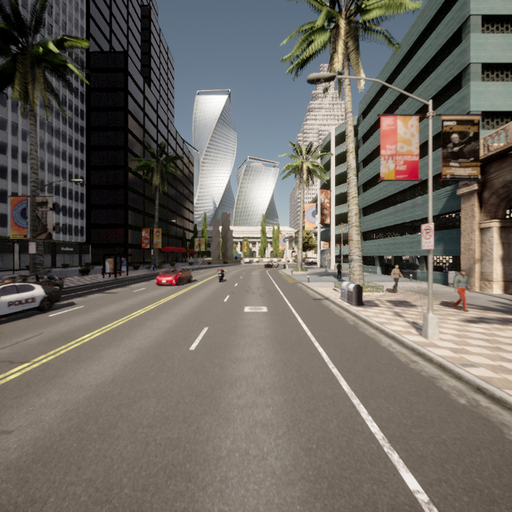
\includegraphics[width=0.85cm]{figures/fig1_thumbs/rgb.png}};
\draw[cRGB, line width=0.6pt] (ti.south west) rectangle (ti.north east);
\draw[trained, rounded corners=1.2pt] (15.0,1.0) rectangle (16.35,1.7);
\node[ttl] at (15.675,1.35) {Model $\ell$};
\node[inner sep=0pt] (tp) at (17.25,1.35) {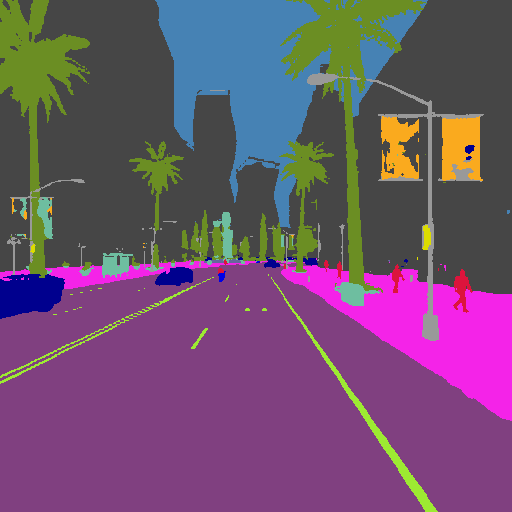
\includegraphics[width=0.85cm]{figures/fig1_thumbs/pred.png}};
\draw[ink, line width=0.5pt] (tp.south west) rectangle (tp.north east);
\draw[flow] (ti.east) -- (15.0,1.35);
\draw[flow] (16.35,1.35) -- (tp.west);
\node[sub, anchor=north, align=center] at (15.675,0.82) {one pass; no teacher,\\no degradation, no extra cost};
\end{tikzpicture}
